\documentclass[a4paper,9pt]{report}
\usepackage[utf8]{inputenc}
\usepackage[parfill]{parskip}
\usepackage[dutch]{babel}
\usepackage[natbibapa]{apacite}
\usepackage[font={small, it}]{caption}
\usepackage{graphicx}

\graphicspath{ {images/} }

% Use case definitie %
\newcommand\tabularhead[1]{
\begin{table}[h]
  \caption{Use-case: #1}
  \begin{tabular}{|p{0.3\linewidth}|p{0.7\linewidth}|}
    \hline
    \textbf{Use-case} & \textbf{#1} \\
    \hline}

  \newcommand\addrow[2]{\textit{#1} &#2\\ \hline}

  \newcommand\addmulrow[2]{ \begin{minipage}[t][][t]{2.5cm}\textit{#1}\end{minipage}% 
     &\begin{minipage}[t][][t]{8cm}
      \begin{enumerate} #2   \end{enumerate}
      \end{minipage}\\ \hline}

  \newenvironment{usecase}{\tabularhead}
{\end{tabular}\end{table}}

% Einde use case definitie %

\begin{document}
  \begin{titlepage}
    \begin{figure}
      \centering
      
\includegraphics[width=90mm]{quintor}
      \vspace{1cm}    
    \end{figure}

    {\huge\centering Architectuur\par}
    \vspace{1cm}    
    {\large\bfseries\centering
      Het opzetten van een peer-to-peer netwerk met identiteit \\
      management door middel van Blockchain technologie
    \par}

    \vfill

    \begin{flushleft}
      Jeffrey van Hoven \\
      14068265@student.hhs.nl \\
      \today
    \end{flushleft}
  \end{titlepage}

  \newpage
  \tableofcontents

  \chapter{Inleiding}

Dit verslag is geschreven in het kader van mijn afstudeeropdracht bij Quintor en dient ter beoordeling van de werkzaamheden die uitgevoerd zijn voor de bachelorstudie Informatica aan de Haagse Hogeschool. 

Door de snelle groei van het Blockchain domein heeft Quintor in 2017 in samenwerking met DUO/MinOCW, Groningen Declaration Network, Stichting ePortfolio Support, TNO en Rabobank, het Blockchain Field-lab Education gestart in Groningen. Het Blockchain-lab is opgezet om expertise en kennis uit te wisselen op regionaal, nationaal en internationaal gebied. De oprichting van het Blockchain Field-lab Education heeft er mede voor gezorgd dat Quintor meer kennis wilt opdoen over het Blockchain domein om zo inzicht te krijgen in hoe Blockchain technologie ingezet kan worden binnen vraagstukken vanuit klanten. 

In hoofdstuk 2 is de organisatie beschreven waar het afstudeertraject heeft plaatsgevonden. Vervolgens wordt in hoofdstuk 3 de opdracht gepresenteerd. In hoofdstuk 4 wordt de aanpak van de opdracht onderbouwd en in hoofdstuk 5 wordt de orientatie van de opdracht besproken. In hoofdstuk 6 worden de werkzaamheden van het vooronderzoek besproken waarin de basis van Blockchain technologie ter sprake komt. In hoofdstuk 7 wordt het hoofdonderzoek naar de segmenten Identity Management en Distributed Network in bestaande Blockchain implementaties beschreven. Hoofdstuk 8 presenteert het advies dat gegeven wordt naar aanleiding van het gedane onderzoek. Hoofdstuk 9 beschrijft de totstandkoming van het ontwerp voor de architectuur. In hoofdstuk 10 worden de keuzes die gemaakt zijn voor de indeling van het Proof of Concept beschreven en wordt er kort uitgelicht hoe de realisatie van het Peer-to-Peer netwerk is verlopen. In hoofdstuk 11 wordt er geëvalueerd over de producten, de aanpak, de geselecteerde beroepstaken, het functioneren in het bedrijf en de leerpunten die getrokken zijn uit het project. Tot slot worden er in hoofdstuk 11 aanbevelingen gegeven voor vervolgonderzoek.

  \chapter{Systeem stakeholders en requirements}

\section{Stakeholders}

Er zijn meerdere stakeholders die baat hebben bij de realisatie van dit project:

\paragraph{Quintor} De opdrachtgever en tevens de eigenaar van het project. De organisatie heeft baat bij het opdoen van kennis gedaan door dit project. Tevens zal het de eindgebruiker zijn van het systeem.

\paragraph{Kevin Bos} Heeft belang bij de realisatie van het onderdeel Distributed Network en Identity Management gezien de het gedeelte dat gerealiseerd wordt hem samen dient te werken met de componenten die voorgesteld zijn binnen dit document.

\section{Requirements}

\subsection{Business rules}
\begin{tabular}{|p{1.1cm}|p{11cm}|}
  \hline
  BR01 & Berichten dienen van type req(uest), inv(entory), data en auth(entication) te zijn. \\
  \hline
  BR02 & Transactietypes zijn: account -- om een account te registreren in het netwerk, data -- arbitraire data dat nog niet gedefinieerd is. \\
  \hline
\end{tabular}

\newpage
\subsection{Functional requirements}

\begin{tabular}{|p{1.1cm}|p{8cm}|p{3cm}|}
  \hline
  \textbf{Id} & \textbf{Beschrijving} & \textbf{Prioritering} \\
  \hline
  FR01 & Als gebruiker wil ik een transactie kunnen aanmaken. & Must have \\
  \hline
  FR02 & Als gebruiker wil ik mijn data kunnen synchroniseren. & Should have \\
  \hline
  FR03 & Als gebruiker wil ik connectie kunnen leggen met een deelnemer uit het Peer-to-Peer netwerk. & Must have \\
  \hline
  FR04 & Als gebruiker wil ik mijn openstaande connecties kunnen inzien. & Could have \\
  \hline
  FR05 & Als gebruiker wil ik kunnen toetreden in het Peer-to-Peer netwerk. & Must have \\
  \hline
  FR06 & Als gebruiker wil ik een block kunnen aanmaken. & Must have \\
  \hline
  FR07 & Als beheerder wil ik een gebruiker kunnen aanmaken. & Must have \\
  \hline
\end{tabular}

\subsection{Non-functional requirements}

\begin{tabular}{|p{1.1cm}|p{8cm}|p{3cm}|}
  \hline
  \textbf{Id} & \textbf{Beschrijving} & \textbf{ISO} \\
  \hline
  NFR01 & Het systeem dient om te kunnen gaan met deelnemers die de performance van het Peer-to-Peer netwerk proberen te verstoren. & Securability \\
  \hline  
  NFR02 & Het systeem dient om te kunnen gaan met het vervalsen van transacties. & Securability \\
  \hline
  NFR03 & Het systeem dient makkelijk uitgebreid te worden door de kerncomponenten modulair op te stellen. & Maintainability \\
  \hline
  NFR04 & Het systeem dient rekening te houden met protocol updates, en dient interactie met verouderde versies niet te ondersteunen. & Maintainability, Securability \\ 
  \hline
  NFR05 & Het systeem dient makkelijk ingezet te kunnen worden. & Deployment \\
  \hline
\end{tabular}
  \chapter{Architectuur views}

\section{Context view}

De contextweergave van het systeem beschrijft de relaties, afhankelijkheden en interacties tussen het systeem en zijn omgeving (de mensen, systemen, en externe identiteiten waarmee het communiceert).

\begin{figure}[h]
  \centering
  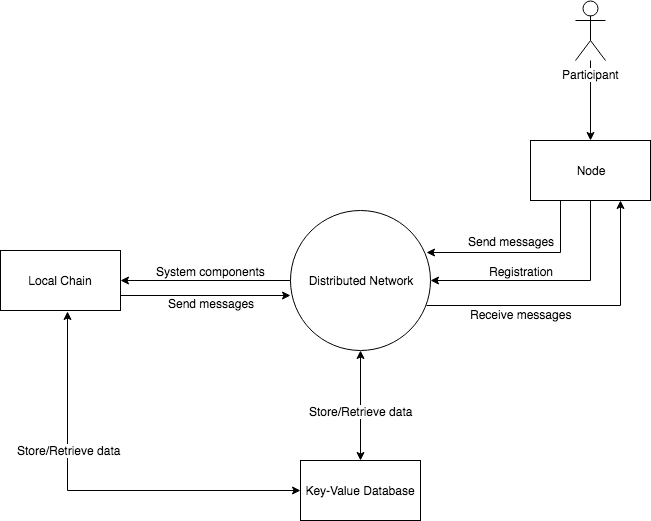
\includegraphics[width=0.7\textwidth]{Context_Diagram}
  \caption[Context Diagram] {
    Context Diagram waarin de interacties te zien is tussen het systeem en zijn omgeving.
  }
\end{figure}

De gebruiker draait een Node die gebruik maakt van het Peer-to-Peer netwerk om berichten te versturen. Een van de berichten is specifiek weergegeven aangezien het gaat om de registratie van een nieuwe gebruiker in het systeem. Het Distributed Network maakt gebruik van entiteiten uit de Local Chain om de benodigde data te versturen. Zowel het Local Chain gedeelte als het Distributed Network maken gebruik van een Key-Value database om data op te slaan. In het geval van het Distributed Network gaat dit om informatie over connecties.
\section{Logical view}

\textit{In de logische weergave wordt de architectuur benaderd vanuit het oogpunt van de eindgebruiker. Hierin komen de functionaliteiten van de verschillende componenten aan bod om de functionaliteit te ondersteunen.}

\begin{figure}[h]
  \centering
  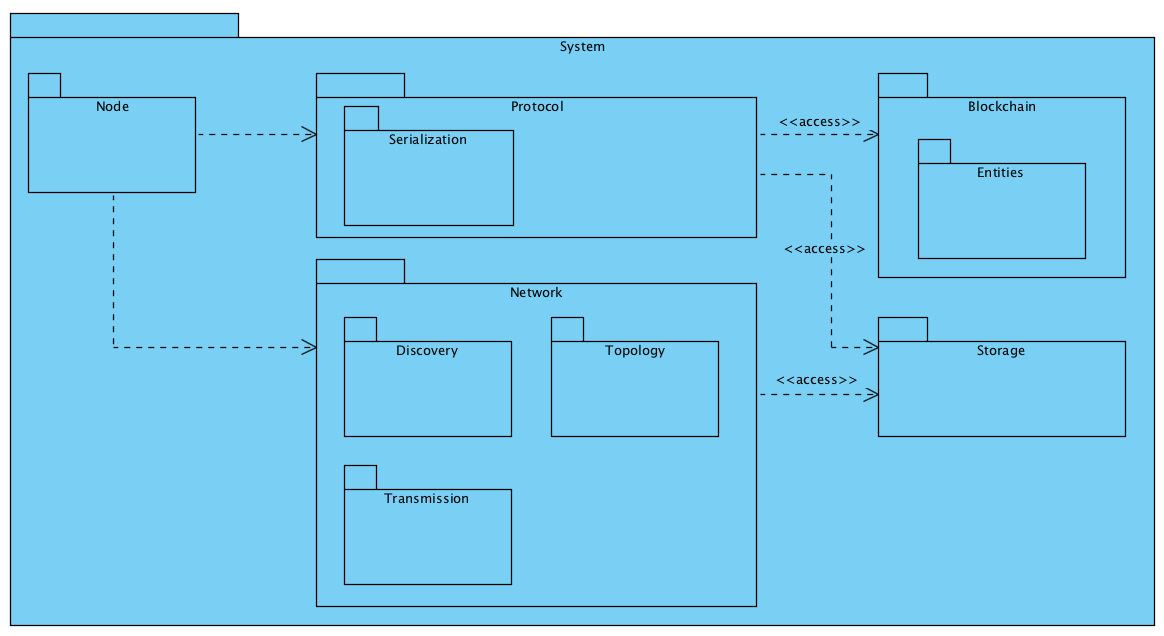
\includegraphics[width=1\textwidth]{package_diagram}
  \caption{Overzicht van het systeem}
  \label{diagram:package}
\end{figure}

In fig. \ref{diagram:package} is een overzicht te zien van de verschillende onderdelen van het systeem. De node is het startpunt van het systeem en maakt gebruik van een protocol specificatie om entiteiten uit de Blockchain op te maken in berichten die geschikt zijn voor het geïmplementeerde protocol. 

Daarnaast maakt het gebruik van de netwerk specificatie om het toe te treden, de topologie te creëren en berichten die gemaakt zijn door het protocol te versturen.

Op de volgende pagina's zijn de verschillende componenten in detail gemodelleerd.

\newpage
\begin{figure}[h]
  \centering
  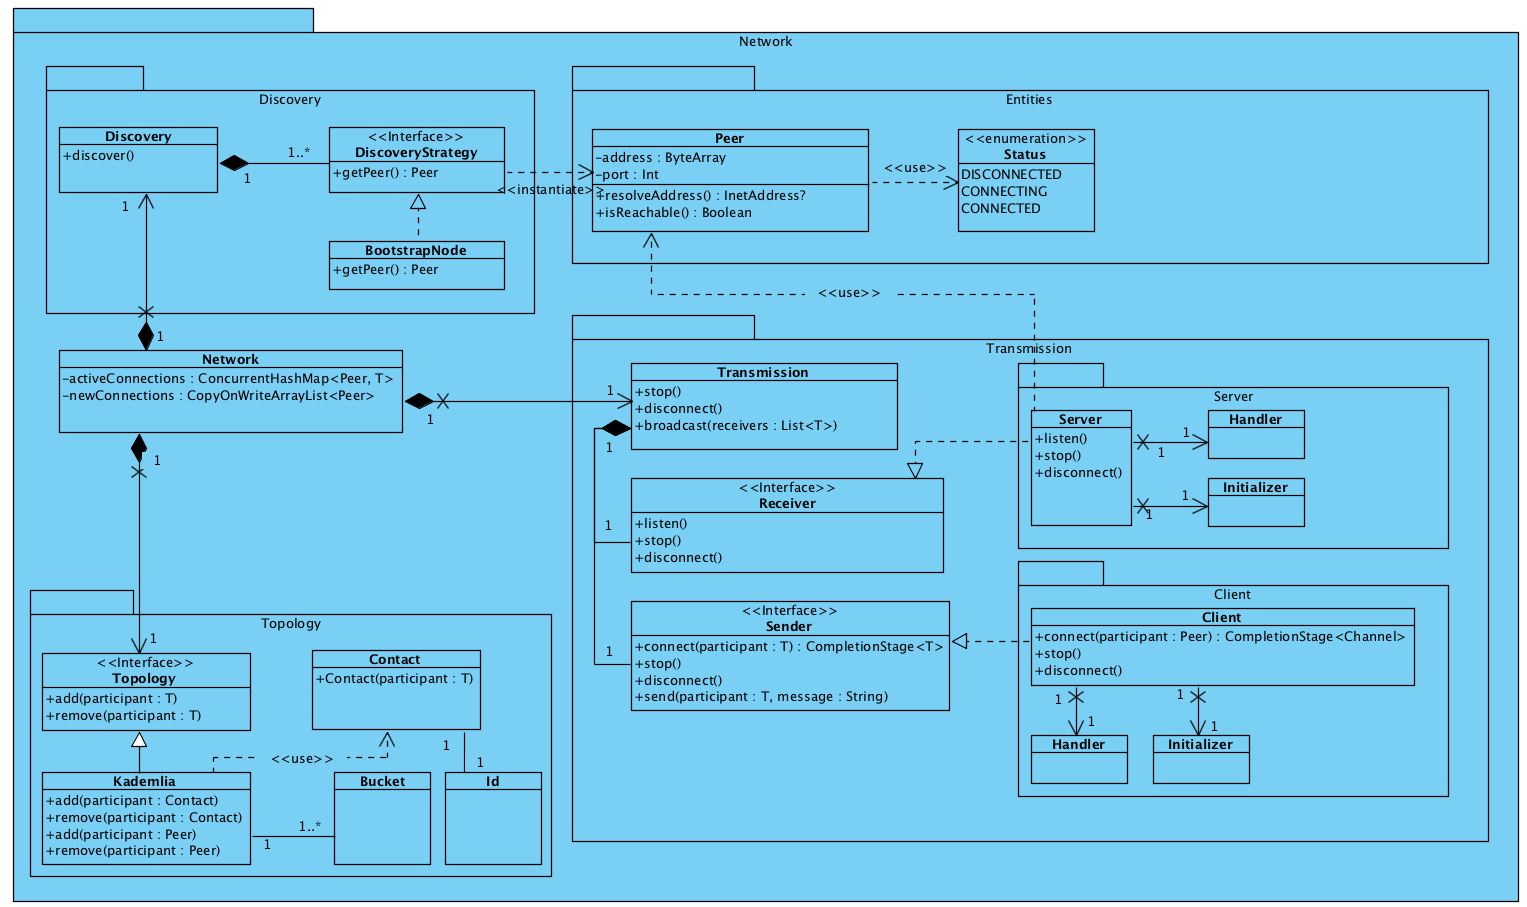
\includegraphics[width=1\textwidth]{network}
  \caption{Gedetailleerd overzicht van het Network component}
  \label{diagram:network}
\end{figure}

In fig. \ref{diagram:network} is een gedetailleerd overzicht te van van het Network component. Het Discovery component is verantwoordelijk voor het uitvoeren van het Peer Discovery Protocol dat gebruikt wordt ten tijde van het toetreden van het netwerk. Er wordt hierbij gebruik gemaakt van een strategie, namelijk het opzoeken van een BootstrapNode. 

Het Topology component is verantwoordelijk voor de structuur van het netwerk. Dit is modulair opgebouwd zodat het makkelijk gewisseld kan worden door een andere implementatie. De default topology is het Kademlia protocol.

Het Transmission component is verantwoordelijk voor het versturen en ontvangen van berichten. Dit is opgesplitst in een \textit{Receiver} en \textit{Sender} interface zodat het niet protocol specifiek geïmplementeerd hoeft te zijn.



\newpage
\section{Development view}

\textit{De development weergave illustreert het systeem van een programmeur perspectief en omvat het Software Management gedeelte.}

\begin{figure}[h]
  \centering
  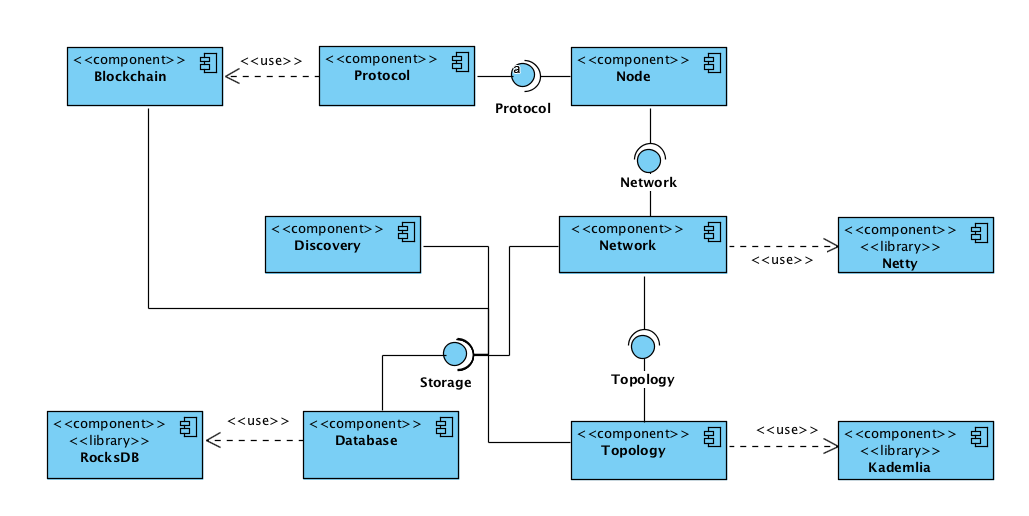
\includegraphics[width=1\textwidth]{component_diagram}
  \caption[Component Diagram] {
    Component Diagram waarin de diverse componenten en de samenwerking daartussen te zien is.
  }
  \label{diagram:component}
\end{figure}

In fig. \ref{diagram:component} is het component diagram te zien waarin de kerncomponenten van de applicatie staan. Hieronder zijn alle component individueel besproken:

\begin{itemize}
  \item \textbf{Blockchain}
  \\ Het Blockchain component bevat de logica en cryptografie om de structuur van een Blockchain op te bouwen. Een belangrijk onderdeel van het Blockchain component zijn de identiteiten die benodigd zijn voor de communicatie tussen verschillende participanten van het netwerk.
  \item \textbf{Protocol}
  \\ Het Protocol component stelt de regels op met betrekking tot het gebruik van de Blockchain data.
  \item \textbf{Node}
  \\ Het Node component bevat de functionaliteit waarmee de eindgebruiker kan interacteren.
  \item \textbf{Network}
  \\ Het Network component is een encapsulatie van de verschillende componenten die hier deel van uitmaken. Het is verantwoordelijk voor het opzetten van het gehele Peer-to-Peer netwerk.
  \item \textbf{Discovery}
  \\ Het Discovery component bevat de Peer Discovery mechanisme die gebruikt om toe te treden in het netwerk.
  \item \textbf{Topology}
  \\ Het Topology component bepaald de infrastructuur van het Peer-to-Peer netwerk.
  \item \textbf{Database}
  \\ Het Database component bevat de logica om te interacteren met de gekozen database implementatie.
\end{itemize}
\section{Physical}
\section{Process}



  \bibliographystyle{apacite}  
  \setlength\bibsep{\baselineskip}  
  \bibliography{bronnen}
\end{document}

